%======================================================================

\chapter{Model Specification}\label{ch:model-specification}

In order to model such a system, we incorporate the notation most frequently seen in the
study of palm calculus \cite{baccelli_elements_2003}. Most importantly, assuming we delegate a probability space $(\Omega, \mathcal{F}_{t}, \mathcal{F}, P)$ with the measurable flow $\{\theta_{t}\}$ which is $P/\theta_{t}$ invariant (i.e., Ergodic such that $\theta_{t}M = M \text{  for some } M \in \mathcal{F} \Rightarrow P(M) \in \{0,1\}$), then the arrival process $A$ can be associated with the flow.
In a system with Markovian arrivals, the counting measure associated with the flow would necessarily be Poisson;
other so-called counting processes wherein inter-arrivals are determined by random or even deterministic periods of time can be used. Inter-arrival times (for arrival $n$ occurring at $T_{n}$), regardless of the generating process, shall be denoted
\[\tau_{n} = T_{n+1}  - T_{n}, n \in \mathbb{N}.\]
Intensities (even if non-Poisson) will be denoted $\lambda = E(A((0,1])))$ for arrival process $A$, being interpreted as the intensity of a process moving a state (i.e., counting an additional element) within unit time.
\begin{definition}[Marked Process]
    For each job which enters the system, they can be ``marked" by a series of random variables defining their behaviour within the system \cite{baccelli_elements_2003}. In general, for the systems we shall consider, we consider the marked process $\sigma_{n}$ as being the required service of arrival $n$ and the marks $T_{n}$ as its time of arrival.
    The tuple \[(T,\sigma)_{n}, n \in \mathbb{N}\] will therefore be used to mark the $n$th job.
    We shall extend this notation, however, to include sets;
    for a set of jobs $\eta$, wherein each element has their own arrival time,
    \[(T, \sigma)_{\eta} = \{(T,\sigma)_{n}\}_{n \in \eta}.\]
\end{definition}

In a simple $G/M/c$ queue, as discussed before, the double $(T,\sigma)_{n}$ would be sufficient for reducing the problem into a deterministic one.
In our case, given that jobs can find their status in the system tied to the behaviour of their replicas, we must append a marking to track this phenomenon.
As a matter of fact, we instead move to marking the queues as was done by \cite{bramson_asymptotic_2012} to prove the conjecture in the case of Join-The-Shortest-Queue($d$) systems, although with an additional job dependency term.

\begin{definition}[Job Dependency Graph: Finite Case]
    \hfill \\
    The \textbf{Job Dependency Graph}, $G_{t}=(V,E)_{t}$, is held constant between the events of arrivals and job completions, where an edge is drawn between two nodes if and only if they are job-dependent. Moreover:

    \begin{enumerate}
        \item Movement in a queue requires \textit{appropriate} redrawing of graph.
        \item $G_{t}$ is stochastic with law in $\text{Pr}(\Omega, \mathcal{F}_{t})$.
        \item Maximal system queue size is bounded, $\sup_{n \in \chi}z_{n}(t):=\nu(t).$
    \end{enumerate}
    ``Appropriate redrawing" in this case means:
    \begin{enumerate}
        \item The graph is redrawn to reflect movement within each queue (moving due to job completions or arrivals).
        \item $G_{t}$ can depend only on $G_{s}, s <t$, and other current values of $X_{t}$ (denote these other values by $\tilde X_{t}$) and is such that \[P(G_{t}|\tilde X_{t}, \{G_{a}\}_{a \in S})=P(G_{t}|\tilde X_{t}, G_{\max(S)})\]
        for any set $S$ such that $ S \subset [0,t)$.
    \end{enumerate}
    \label{dep1}
\end{definition}
\begin{definition}[Job Dependency Matrix: Finite Case]
    \hfill \\
    The \textbf{Job Dependency Matrix} is an adjacency matrix (non-unique but one-to-one) for $G_{t}$. Specifically,
    \begin{align}
        \rho(t)\equiv \rho(G_{t})=
        \left[  \enskip
        \begin{matrix}[c|c|c|c]
            B_{1,1}  & B_{1,2}  & \dots & B_{1,\nu}\\
            \hline
            \vdots & \vdots & \vdots &\vdots  \\
            \hline
            B_{\nu,1}  & B_{\nu,2} & \dots   & B_{\nu,\nu}\\
        \end{matrix} \enskip \right]
        \label{rho}
    \end{align}
    is a blocked matrix such that sub matrix
    \[B_{i,j}= [b_{q,m}]_{q,m \leq N} = \begin{cases}
                                            1, \substack{if \text{ queue } q \text{ in row } i \text{ is connected in } G_{t} \\ \text{ to queue } m \text{ in row } j}\\
                                            0, \text{otherwise}
    \end{cases}\]
    where connections between jobs occur if and only if the completion of one job implies the removal of all other connected jobs from the system.
    \label{jdf}
\end{definition}

While complicated in the above form, this graph merely draws an edge between jobs of separate queues while tracking their current place in their respective queues. Because at most one event can happen in infinitesimal time (i.e., an arrival or departure), the assumptions merely state that between any two events this graph shall not need to be redrawn. Extending this notion, one can iterate such a procedure indefinitely, viewing the resultant infinite graph as one where jobs are joined by hyperedges if and only if there exists an element of a set of replicas in each of the queues. In other words, one can represent queues which are connected by means of having replicas of the same jobs enqueued within them by viewing each as a node connected with a hyperedge; we will call queues related by such a hyperedge members of a \textit{replica class} . Thus, Definition \ref{dep1} can be represented more succinctly in a hypergraph form, allowing one to represent the cavity process studied in \cite{Hellemans}.

\begin{definition}[Hypergraph Representation of the Dependency Matrix]
    \hfill \\
    By collapsing edges as jobs and vertices as servers, all connected subgraphs of $G_{t}$ can be thought of as incident nodes with edges $i_{1}, \dots i_{j}$ for $j<d$, representing connected jobs. This gives us now only as many nodes as there are currently servers. Such a representation for $G_{t}$ will be denoted by $\mathcal{G}_{t}$. See Figure~\ref{fig:hyper} for a visual representation.
\end{definition}

\begin{figure}
    \centering
    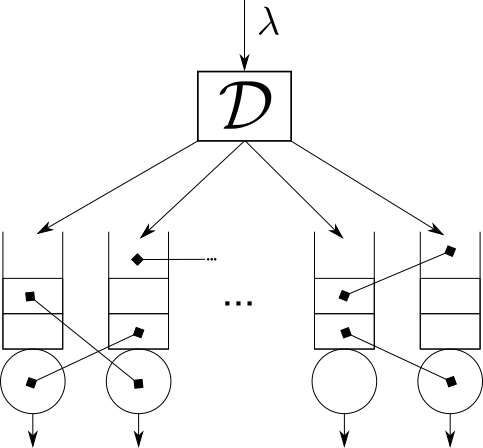
\includegraphics[scale=0.5]{systemredun}
    \caption{A graphical representation of queues with replicated jobs as hyperedges.}
    \label{fig:hyper}
\end{figure}

When one creates the infinite graph iteratively, it is meant that one could view the graph described in Definition \ref{dep1} as an embedding into a larger graph by merely considering more queues or a larger maximal queue size at any finite time $t$, corresponding to the adding of an additional column or row of vertices, respectively. Building a metric on an infinite graph space simplifies the matter of quantifying convergence in terms of $N$ significantly because all possible finite embeddings can be expressed in the same space as $N\rightarrow \infty$. Thus, let us consider \[\mathbb{E}:= \{\text{locally finite graphs}\}.\] Now, extending the notation of \cite{bramson_asymptotic_2012}, we can fully describe the marked process for queues with general service times.
\begin{definition}[State Space With Redundancy]
    \hfill \\
    With $\psi$ as $[n]$ or $\mathbb{N}$, $\rho(\cdot)$ denoting the matrix representation of a graph, and $\mathbf{X}^{\psi}$ denoting a system of $\psi$ parallel queues,
    let us assign $X_{n}(t)$ to the $n$th queue of the $\psi$-indexed possible queues such that $X_{n}(t)$ follows the $n$th marginal distribution of $\mathbf{X}^{\psi}$.
    Adapting the notation of \cite{bramson_asymptotic_2012}, we assign state spaces to $X_{n}$ and $\mathbf{X}^{\psi}$ as follows:
        \[X_{n}(t)\in (\mathbb{N},\left(\mathbb{R}^{+}\right)^{3},\rho(\mathbb{E})):=\mathcal{E}^{(\psi)}_{n}\]
    and
        \[\mathbf{X}(t) \in \{\mathcal{E}^{(\psi)}_{n}\}_{n \in \psi} := \mathcal{E}^{(\psi)},\]
    such that $X_{n} = (z_{n}(t), w_{n}(t),l_{n}(t),v_{n}(t),A(t))$ where
    \begin{enumerate}
        \item $z_{n}(t) \in \mathbb{N}$ denotes queue size,
        \item $ w_{n}(t) \in \mathbb{R}^{+}$ denotes workload,
        \item $\ell_{n}(t) \in \mathbb{R}^{+}$ denotes the amount of service time spent on job currently with server,
        \item $v_{n}(t) \in \mathbb{R}^{+}$ denotes the time remaining for job in server,
        \item $A \in \rho(\mathbb{E})$ is a representation of the graph.
    \end{enumerate}
    \label{def:spec}
\end{definition}


%======================================================================
%\begin{definition}(Hypergraph Representation of the Dependency Matrix)
%By collapsing edges as jobs and vertices as servers, all connected subgraphs of $G_{t}$ can be thought of as incident nodes with edges ${i_{1}, \dots, i_{j}}_{j<d}$ representing connected jobs. This gives us now only as many nodes as there are currently servers.
%\end{definition}
%
%Following with \cite{newgraph} for the remainder of the paper, the following assumption is made (and indeed can always be constructed):
%$G_{t}$ has the rooted graph component $(G_{t},o)$ for $o \in E(G_{t})$ being an arbitrary, particular element. We call $[G_{t},o]$ the class of graphs root-isomorphic (that is, isomorphic with respect to the root) to $(G_{t},o)$.  Also define $G_{t}^{*}$ to be the class of rooted locally finite graphs on $G_{t}$. Define the metric $\alpha := \sup \{r \in \mathbb{N}| r = \text{minimum length of paths connecting two graphs' roots}\}$ and $d = \frac{1}{1+\alpha}$ as another; both exist on $G^{*}_{t}$ and it can be shown that $G^{*}$ is seperable and complete \ref{newgraph}. $U(G)$ defines the distribution on $G^{*}$ obtained by choosing a random vertex as a root. Lastly, $[N]$ will be used to denote a vertex set for a graph $G_{t}^{N}\in(G_{t}^{N})_{N \in \mathbb{N}}$.
%
%\begin{definition}(Spectral Measure, \cite{hualiue2015})
%\[\mu_{G, o}(A)=\frac{1}{\theta_{o}}\left\langle P_{A} \delta_{o}, \delta_{o}\right\rangle, \quad \forall A \subset[0,2].\]
%\end{definition}
%One can show that this generalizes the usual spectral measure on finite graphs. We now can introduce a relevant graph pseudo-metric.
%\begin{definition}(Wasserstein Mean Distance)
%With the usual Wasserstein distance being defined as \[d_{p}^{W}(\mu, v):=\left(\inf _{\pi \in \Pi(\mu, v)} \int_{| 0,2] \times | 0,2\}} d(x, y)^{p} d \pi(x, y)\right)^{1 / p}\] for $\pi$ being a measure of the joint distribution, the distance taken over the expectation of each measure is the Wasserstein Mean Distance.
%\end{definition}
%
%The prior definitions are required in order to be able to quantify convergence; the remainder of the paper shall concern detailing how this is achieved. Following Bramson (2012), a modification allows us a means to prove convergence through coupling. In our case, we merely need to only choose an initial condition where a workload-based loss function is minimized.
%
% \begin{definition}[\textit{Queued Loss}]
% \\~\\
% \[W^{(l)}_{n}:= \sum_{i\in[F]}\min_{j\in [J]}(V_{j_{i}}),\]
% Where $l$ denotes the index in the coupling, $[a]=\{1, \dots, a \}$, $V_{a}$ denotes the time (workload) that the $a$th job has remaining for processing, $F$ denotes the size of queue $n$, and $J$ is the number of copied jobs in the system for the $i$th job in the queue.
% \end{definition}
% \begin{definition}[\textit{Queued Loss Domination}]
% \\~\\
%$W^{(2)}$ is said to dominate $W^{(2)}$ in queued loss at time $t\in [\tau_{i}, \tau_{i+1})$, where $\tau_{i}$ is the $i$th arrival,if
%\[\sup_{A \in [\mathcal{F}_{\tau_{i}},\mathcal{F}_{\tau_{i+1}}),n \in [N]}W^{(1)}_{n} \leq \inf_{A \in [\mathcal{F}_{\tau_{i}},\mathcal{F}_{\tau_{i+1}}),n \in [N]}W^{(2)}_{n}.\]
%In the above case, we take $W^{(l)}_{n}\equiv W^{(l)}_{n}(A)$ as in the usual measure-theoretic definition of a random variable. We denote the case where the above holds true with the partial ordering $W^{(2)}\succ W^{(1)}$.
% \end{definition}
% An important result which follows is a connection to job-independent case.
% \begin{theorem}
% \[\sup_{A \in [\mathcal{F}_{\tau_{i}},\mathcal{F}_{\tau_{i+1}})}W^{(l)}_{n}=W_{n}^{(l)}|_{J=1}.\]
% \end{theorem}
% The above proposition is actually trivial given that between Markov arrivals and without any connections, the system behaves in the usual PDMP manner on workload, decreasing linearly. If one were to add a connection, however, should that connected job reach the server in its corresponding queue while in queue $n$ it waits, $W_{n}^{(l)}$ will decrease faster but cannot ever increase (until an arrival). This gives us the smallest possible value for the queued loss of system 2.
%
% \begin{theorem}[\textit{Queued Loss Domination is Preserved Stochastically}]
% \\~\\
% Under the standard ordering (Bramson, 2012) with queued loss in place of workload,
% \[\forall s>0, W^{(2)}_{t=0}\succ W^{(1)}_{t=0} \Rightarrow W^{(2)}_{t=s}\succ W^{(1)}_{t=s}. \]
% \label{loss}
% \end{theorem}
% \textit{Proof.}
% \\~\\
% At time $0$ we choose $W^{(2)}$ in such a manner that it has the same jobs and workloads for each job but without any connections on the graph. That is, we have \[W^{(2)}:=\underset {n \in [N]}\sup W^{(1)}|_{J=1}.\] At time $\tau_{1}$, a job arrives and, due to the coupling, consults the same selection set at $W^{(1)}$ and $W^{(2)}$, which is of size $D$. Without loss of generality, let us order the queues within each selection set with index $n \in [D]$. Independently, in each space, a job is copied and placed into the queues for which $W^{(l)}_{n} \leq R$, with $R$ denoting the threshold of the routing algorithm. Define $[D_{\text{send},l}]\subset[D]$ to be the queues for which, out of those queried, the threshold permitted copying. By setting $W^{(2)}$ as we had, its minimum queue in the $[D]$ is at least as large as the maximum selected in $W^{(1)}$, giving $ [D_{\text{send},2}]\subset [D_{\text{send},1}]\subset[D]$.
%
% We must now show that the result continues to hold between all arrival times. Consider $T=\inf\{s>0:W^((2))_{t=s}\not \succ W^{(1)}_{t=s}\}$. Just as in the case of Bramson (2012), the only possible discrepancy will occur an arrival occurs in system 1 at queue $n_{2} \not = n_{1}$, where it arrives in system 2, at $T$. At time $T^{-}$, we must have $W^{(1)}_{n_{1}}\leq W^{(2)}_{n_{1}}$ and $W^{(1)}_{n_{2}} \leq W^{(2)}_{n_{2}}$ as, of course, the ordering still is held at this point. If an arrival has workload $A$, and consults the same selection set, $M$, we must have the discrepancy due to  $W_{n_{1}}^{(1)} \leq R$ \quad \qedsymbol.
%
%In the context of exchangeability, we incorporate various notations. Importantly, the notation developed in Adan et al. (2018) and employed in a similar context by Cruise et al. (2020) can be borrowed immediately to model the system at hand. Namely, we shall henceforth consider the $\mathcal{D}_{Thresh}$ system as a hypergraph of form $(\mathcal{V},\mathcal{E})$ wherein vertices represent servers and hyperedges a collection of dependent jobs (see Adan et al. (2018) for a visual example). Similarly, we shall refer to a customer class (a set of dependent jobs) as $c^{i}$ for $i$ referring to the $i$th job to arrive to the system (before cloning). This hypergraph model allows us to employ the notion of exchangeability described by Austin (2008, 2013).
%
%\begin{definition}[$(T,\Gamma)$ \textit{Exchangeability (Austin, 2008)}]
%\\~\\
%If $\Gamma$ is a group of permutations on $Y$ preserving the partition $\cup_{i=0}^{k}y_{i}$, then the joint law over the partition ($\{\pi_{y_{i}}_{i \leq l}\}$) is considered $(Y,\Gamma)$ exchangeable if the joint distribution is invariant under each of $\Gamma$'s rearrangements. That is to say, all rearrangements are equal in distribution.
%\end{definition}
%
% The obvious application under our model will be in applying this notion to a dependent group in place of the aforementioned arbitrary $y_{i}$ values. Austin (2008; Theorems 2.5 and 3.1) also proves the integral result of asymptotic independence existing between vertices (queues) in a proof by kernel construction. The "replica trick" suggested by Bramson et al, (2013) as well as Hellemans et al., (2019) is explicitly related to the general case of arrays in the later work of Austin (2014, Proposition 2.1). Of course, an array is merely a generalization of a hypergraph, making this method immediately applicable to our problem.
%
%%\begin{proposition}[\textit{Preservation of Ordering at Equilibrium}]
%%Referring to $\epsilon_{i}$ as the equilibrium distribution (that is the distribution for asymptotic $t$) for space $i \in {1,2}$ as in Theorem \ref{loss}, if $\epsilon_{i}(0)$ is $\{d,\dots,0\}=[d]$-exchangeable, then $\epsilon_{i}(t)=\epsilon_{i,\pi}(t) \forall t$
%%\end{proposition}
%
%\begin{lemma}
%\label{lem:build}
%For any infinite $d$-echangeable (and thus $d$-complete) hypergraph, one can build it from a $\{d,\dots,0\}=[d]$-exchangeable finite hypergraph (uniquely, P-as).
%\end{lemma}
%\textit{proof}
%This follows immediately from the replica trick; a rank $d$ hypergraph (as it should be in order to be $[d]$-exchangeable), can be represented as the family $(X_{e})_{|e| \leq d}$ where $X_{e}$ is a particular set of vertices. In this case, one would consider the hyperedge to be each at-most-$d$ collection of vertices. Following Austin (2014), for product measure (and thus, a measure for an exchangeable random variable) $\mu$, by means of coupling/replicating, one can build the double $((X_{i,e})_{i \in \mathbb{N},e \in \mathbb{N}^{\leq d}},(X_{e})_{e \in \mathbb{N}^{\leq d}})$. As such, the rest of the proof follows directly as in Austin (2014). \quad \qedsymbol
%
%\begin{lemma}
%\bold{note - redid proof to this one; typing it up and borrowed extensively from Austin 2008. This way avoids the need to use Feller continuity which is tedious and allows us to avoid another long constructive proof and cut to the chase). Also removes trhe need for another proof altogether due to the fact that I previously had to jump through some hoops to deal with the non-equality but this way gives it exactly as needed}
%Let $\varepsilon_{1} \overset{\mathcal{P}}{\leq} \varepsilon_{2} \iff \exists \pi \in \text{Sym}(W_{2}): W_{1}(\omega) \succ W_{2,\pi}(\omega), \forall \omega \in \mathcal{F}$. If $[d]$-exchangeable, then there exists mappings $G,G'$ such commutivity is observed as in Figure \ref{fig:comm}.
%\begin{figure}
%    \centering
%\begin{tikzpicture}
%	\begin{pgfonlayer}{nodelayer}
%		\node [style=invisibox] (0) at (0, 0) {$(\Omega,\mathcal{F}_{t}, \mathcal{F},  P)^{\mathcal{P}[d]}$};
%		\node [style=invisibox] (1) at (4, -3) {$(\Omega,\mathcal{F}_{t}, \mathcal{F},  P)^{\mathcal{P}[d]}$};
%		\node [style=invisibox] (2) at (-4, -3) {$(\Omega,\mathcal{F}_{t}, \mathcal{F},  P)^{\mathcal{P}[d]}$};
%		\node [style=invisibox] (3) at (0, -6) {$\mathbb{R}^{[d]}$};
%		\node [style=cir] (4) at (2, -1.5) {$\hat{G}'$};
%		\node [style=cir] (5) at (-2, -1.5) {$\hat{G}$};
%		\node [style=cir] (6) at (-2, -4.5) {$\hat\varepsilon_{2}$};
%		\node [style=cir] (7) at (2, -4.5) {$\hat\varepsilon_{2,\pi}$};
%	\end{pgfonlayer}
%	\begin{pgfonlayer}{edgelayer}
%		\draw [style=larrow] (1) to (0);
%		\draw [style=larrow] (2) to (0);
%		\draw [style=larrow] (3) to (2);
%		\draw [style=larrow] (3) to (1);
%	\end{pgfonlayer}
%\end{tikzpicture}
%
%
%    \caption{Commutivity Diagram}
%    \label{fig:comm}
%\end{figure}
%\end{lemma}
%
%\textit{Proof}
%Recall from Lemma \ref{lem:build} that for any graph, one can construct it in terms of finite graphs uniquely. Thus, for different $\varepsilon_{1}, \varepsilon_{2}$ one can build from $W_{1}(0), W_{2}(0)$ respectively in this manner to satisfy. Taking $\varepsilon_{i}$ to be empirical means that, as Austin (2008, section 6.1) shows, $W_{i}(0)$ must be $[d]$ exchangeable for $i \in \{1,2\}$ implying that the dual $(W_{1}(t),W_{2,\pi}(t))$ must be due to coupling.





